% -- Deckblatt.tex -----------------------------------------------------------
%
%   Gestaltung des Deckblattes der Bedienungsanleitung:  
%   - Einbinden und formatieren der Logos
%   - Bezeichnungen befinden sich in 'Meta.tex'   
% ------------------------------------------------------------------------------

\thispagestyle{empty} % von plain nach empty
\begin{titlepage}
\vspace*{-3cm}% vertikale negative Verschiebung
%%------------------------------------------------------------------------------
%%   Firmenlogo einf�gen
%%------------------------------------------------------------------------------
\begin{figure}[h]
\centering

\includegraphics[width=0.25\textwidth]{schlizbaeda.png}
\end{figure}

\begin{center}
\LARGE{\textbf{\Dokumentart}}\\[1.5ex] 
\Large{\BezeichnungLang}\\[4ex]
%%------------------------------------------------------------------------------
%%   Titel der Bedienungsanleitung
%%------------------------------------------------------------------------------
\noindent\rule[1ex]{\textwidth}{3pt} % vertikaler Strich
%\huge{\textbf{\titel}}\\[1.5ex]      % TITEL DER ARBEIT
\textbf{\titel}\\[1.5ex]              % TITEL DER ARBEIT (lange �berschrift)
\noindent\rule[1ex]{\textwidth}{3pt} 
%\LARGE{\textbf{\untertitel}}\\[6ex]
%\LARGE{\textbf{\art}}\\[1.5ex]
%\Large{im Fachgebiet \fachgebiet}
\\[2ex]

\normalsize
%%------------------------------------------------------------------------------
%%   Bild
%%------------------------------------------------------------------------------
\begin{figure}[h]
\centering
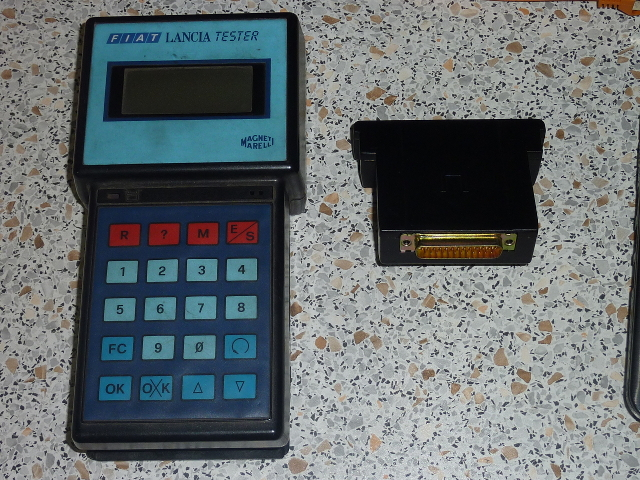
\includegraphics[width=12cm]{Titelbild.JPG}
\end{figure}

%%------------------------------------------------------------------------------
%%   CE und Firmenadresse
%%------------------------------------------------------------------------------
\begin{tabular}{p{3cm} p{8cm} p{3cm}}\\ % die beiden 0.5cm breiten "TabellensSpalten" sind eigentlich latex-unw�rdiges Gepfriemel! Ich kann's aber nicht besser!
\hline
\parbox[c]{75px}{\includegraphics{MagnetiMarelli.png}} & \textbf{Module f�r {\FLTester} programmieren} Datum: 23.10.2016 & \parbox[c]{75px}{\includegraphics{FiatLancia75x75.png}}\\
\hline
\end{tabular}

\end{center}


Diese Anleitung wurde mit dem Textsatzsystem \LaTeX\ erstellt.
%% Das trifft hier nicht zu:
%\textbf{}\\
%Das Bild auf dem Fernsehger�t stammt aus dem Video zu folgendem Musikst�ck:\\
%\texttt{\textbf{Riegler Hias feat. d' Hundskrippln} \textit{Gloana Bauer}} bei 0:15\\
%\url{http://www.hundskrippln.de/#filme}
\end{titlepage}



